\documentclass[tikz, border=5pt]{standalone}
\usepackage{amsmath}

\begin{document}
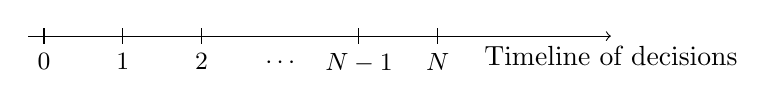
\begin{tikzpicture}

    % Timeline
    \draw[->] (-0.2,0) -- (7.2,0) node[below] {Timeline of decisions};
    \foreach \x in {0,1,2}
    \draw (\x,0.1) -- (\x,-0.1) node[below] {\small \( \x \)};
    \node[below] at (3,-0.15) {\small \( \cdots \)};
    \draw (4,0.1) -- (4,-0.1) node[below] {\small \( N-1 \)};
    \draw (5,0.1) -- (5,-0.1) node[below] {\small \( N \)};

\end{tikzpicture}
\end{document}
